\subsection{Compact prediction ledger}

The main empirical readout table shows only a narrow readout surface. To keep the output
structure visible, \Cref{tab:prediction-ledger} summarizes which output packages belong to which
layer of the paper.

\begin{table}[t]
\centering
\small
\begin{tabularx}{\linewidth}{@{}>{\raggedright\arraybackslash}p{0.18\linewidth}>{\raggedright\arraybackslash}p{0.12\linewidth}YY@{}}
\toprule
Domain & Status & Output package & Source layer \\
\midrule
Carrier packet & Theorem & $E_3\oplus E_2$, $G_{\mathrm{car}}$, $S^+$, $\gamma$, $\bone(N_{\mathrm{fam}},N_\Phi)$ & algebraic normal-form lemma, bosonic-rank corollary, branch-Yukawa rigidity theorem, and half-spinor decomposition \\
Kernel constants & Theorem & $\cthree$, $\phibase$, $\phiz$, $\deltatop$ & exact seam opening and carrier-form closure equation \\
Family / occupancy layer & Theorem & $\Padm$, $F$, $\Oadm=48$, $\deltatop$ & derived corner theorem, admissibility complex, and occupancy corollary \\
Geometric branch & Theorem & $\Phi$, $\Mpl$, $\vgeo$, $R^2$ channel & compact bosonic index plus canonical spectral Einstein functional \\
Renormalized low-energy layer & Theorem & $\GrenTFPT$, charged-current point closure, $v_{\mathrm{phys}}$, pole equations, determinant response, cosmology interface data & charged seam projector lemma, pole-level readout theorem, and renormalized observable hierarchy \\
Transport / flavor closure & Theorem & $Y_f$, CKM, PMNS & residue--winding closure, hard holonomy theorem, and neutrino closure \\
Hadronic / strong-CP closure & Theorem & $\Hhad$, anomaly inflow, $\arg\det M_u=\arg\det M_d=0$ & singlet admissibility plus hard-holonomy determinant suppression \\
Physical observables & Physical observable & $\OphysTFPT$ including pole masses, mixing data, determinant responses, and closed-branch interface packages before late-time cosmology continuation & renormalized observable hierarchy and sector factorization \\
Scheme projections & Scheme projection & $[\Mop(\Tstar)]_{\SchGrp}$ represented by $\Rcmp^{(s)}(\Tstar)$, threshold rows, and ledgers & declared scheme conventions and appendix comparison maps \\
Cosmology block & Appendix continuation & $\Lambda_{\mathrm{IR}}$, $\theta_i$, $N_{\mathrm{DW}}$, $T_R$, and the cosmology interface block & seam transfer, determinant line, scalaron dynamics, and comparison-layer continuation \\
Record layer & Appendix continuation & $\Arec$, $\Aobs$, $\Pred$ & appendix-level record and readout algebra elaboration \\
Appendix continuation & Appendix continuation & E$_8$ scale ratios and modular inner-seam language & appendix-level scale grammar and horizon extension \\
\bottomrule
\end{tabularx}
\caption{Compact prediction ledger for the closed-form presentation after the main-text surface is
split into theorem outputs, physical observables, scheme projections, and appendix continuations.}
\label{tab:prediction-ledger}
\end{table}

\subsection{Empirical readout and kill-test logic}

The present main-text readout surface is no longer intentionally mixed. Its rows now use the
manuscript's closed classes: theorem, physical observable, scheme projection, and appendix
continuation. Carrier algebra and the exact $\alpha$ row remain the sharpest numerically
load-bearing entries, while the former seed-driven rows are now reorganized by sector rather than
counted as one compressed shadow package. The transport block is generative up to physical readout,
the neutrino block is read on the same closed branch, and the electroweak threshold rows appear
only as scheme projections. What remains outside this main-text surface is appendix continuation,
not unresolved theorem load hidden in the core.

\subsection{Residual readout and interface refinements}

The residuals for the restricted six-row readout table are shown in
\Cref{fig:residual-plot}. The carrier-linked electromagnetic, birefringence, and baryon-density
channels all remain within the displayed few-sigma window. The CKM phase is not plotted here
because it is better treated in the operational prediction set and Appendix~\TFPTxref{app:benchmarks}
rather than inside the restricted six-row residual plot.

\begin{figure}[t]
\centering
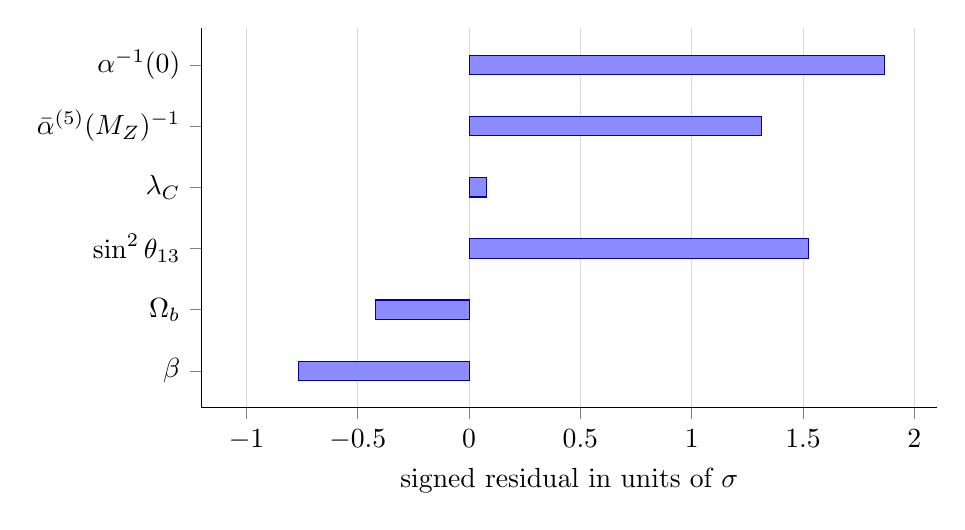
\begin{tikzpicture}
\begin{axis}[
    width=0.9\linewidth,
    height=6.4cm,
    xbar,
    bar width=7pt,
    xmin=-1.2,
    xmax=2.1,
    xlabel={signed residual in units of $\sigma$},
    symbolic y coords={beta,omegab,theta13,lambdac,alphaMZ,alpha0},
    ytick=data,
    yticklabels={$\beta$,$\Omega_b$,$\sin^2\theta_{13}$,$\lambda_C$,$\bar\alpha^{(5)}(M_Z)^{-1}$,$\alpha^{-1}(0)$},
    enlarge y limits=0.12,
    axis x line*=bottom,
    axis y line*=left,
    tick align=outside,
    major grid style={draw=gray!30},
    xmajorgrids=true
]
\addplot[fill=blue!45, draw=blue!70!black] coordinates {
    (-0.768,beta)
    (-0.421,omegab)
    (1.524,theta13)
    (0.078,lambdac)
    (1.315,alphaMZ)
    (1.865,alpha0)
};
\end{axis}
\end{tikzpicture}
\caption{Residual plot for the main empirical readout rows with declared uncertainties.}
\label{fig:residual-plot}
\end{figure}

The principal remaining refinements are therefore specific rather than diffuse:
\begin{itemize}[leftmargin=1.5em, topsep=3pt, itemsep=2pt]
    \item the CKM phase is read from the exact holonomy phase, with only the small-area transport asymptotic kept as a derived expansion,
    \item the nonabelian comparison channels now split into fixed local kernel data and explicit matching functionals, so the remaining sensitivity is numerical rather than structural,
    \item direct-search interface rows remain pressure tests on the closed branch rather than precision residual rows.
\end{itemize}

\section{Technical conventions and data layers}
\label{app:tech}

This appendix collects the technical bookkeeping that supports the boundary-to-carrier presentation but would slow the early main-text flow if placed before the carrier theorem.

\subsection{Relative objects}

The adjective \enquote{relative} is used in one fixed sense throughout the paper: every operator or action is compared to a declared reference object.

\begin{table}[t]
\centering
\small
\begin{tabularx}{\linewidth}{@{}>{\raggedright\arraybackslash}p{0.22\linewidth}YY@{}}
\toprule
Relative object & Definition or schematic form & Role \\
\midrule
$D_{\mathrm{rel}}$ & $D-D_{\mathrm{ref}}$ or a specified relative pair $(D,D_{\mathrm{ref}})$ & fermionic comparison operator \\
$\Gamma_{\mathrm{grav}}$ & $-6\chigeo^2\mathcal E_D+\Gamma_D^{(4)}$ with $\mathcal E_D=\operatorname*{Res}_{s=1}\mathcal Z_{\mathrm{rel}}$ and $\Gamma_D^{(4)}=\operatorname{FP}_{s=0}\mathcal Z_{\mathrm{rel}}$ & canonical spectral Einstein functional from relative residues \\
$\Gamma_{\mathrm{rel}}$ & admissible relative action preserved by the sheet antiunitary involution & strong-CP and reflection-symmetry package \\
$\Ind_{\mathrm{rel}}$ & APS-type index of a relative pair or superconnection package & carrier and bosonic counting \\
$Z_{\mathrm{rel}}$ & $Z_{\mathrm{adm}}[J,\eta,\bar\eta]/Z_{\mathrm{ref}}[0,0,0]$ & normalized admissible generating functional \\
$\Padm$ & $\operatorname*{s-lim}_{\beta\to\infty}e^{-\beta\Kadm}$; factorized form when the elementary projectors commute & operative admissibility selector on the closed branch \\
$\langle W(C)\rangle_{\mathrm{rel}}$ & Wilson observable after subtraction of the declared reference sector & confinement diagnostics \\
$\mathcal H_{\mathrm{rel}}$ & relative Hamiltonian used in admissible-sector minimization & optional record extension \\
\bottomrule
\end{tabularx}
\caption{Conventions on relative objects.}
\label{tab:relative-objects}
\end{table}

\subsection{Layered datum and admissibility}

\begin{construction}[Layered datum]
The technical bookkeeping behind the manuscript uses five levels:
\[
\Tcore^{\mathrm{kin}}
=
\bigl(
\widetilde M\to M,\ \Seam,\ \taudbl,\ \iC,\ D_{\mathrm{ref}},\ D_{\mathrm{rel}},\ f,\ \chiseed
\bigr),
\]
\[
\Tker^\partial
:=
\bigl(
(\mathcal A,\mathcal H,D,J,\Gamma,\taudbl,\iC,\Pprim),\ [u_\Sigma],\ \cthree
\bigr),
\]
\[
\Tker
=
\bigl(
(\mathcal A,\mathcal H,D,J,\Gamma,\iC,\Pprim,\Padm),\ E_3\oplus E_2,\ Y,\ [u_\Sigma],\ \cthree
\bigr),
\]
\[
\Tbridge
=
\bigl(
\mathcal R_{\SM},\ \alpha(0),\ M_Z,\ \{m_c,m_b,m_\tau,m_t\}
\bigr),
\]
\[
\Tcomp
=
\left(
\begin{array}{l}
(\mathsf{Adm},\Kadm,\Padm),\ (\chigeo,\mathcal B_{\mathrm{rel}},\mathbb A_{\Seam}),\ (F,T),\\
(U_6,D_y,\mathcal Y_y^{(\varepsilon)},\epsilon_f),\ (Z_{\mathrm{rel}},\Theta,\Hrel,\Vadm),\\
(\Arec,\Aobs,\Pred)
\end{array}
\right).
\]
Here $\Tker^\partial$ is the primitive boundary kernel, while $\Tker$ is the derived theorem-level
post-carrier kernel reconstructed from the joint discrete datum and the full selector.
\end{construction}

Thus $\Tcore^{\mathrm{kin}}$ is the appendix bookkeeping rewrite of the primitive kinematic
scaffold, while $\mathsf{Adm}$ first enters the layered datum only at closure level through
$(\mathsf{Adm},\Kadm,\Padm)$. When an almost-commutative factorization
$\mathcal H\cong L^2(\widetilde M,S)\otimes\Hint$ is chosen, $S$ and $\Hint$ refer to that
factorization and are not additional entries in $\Tcore^{\mathrm{kin}}$.

Optional horizon and far-downstream E$_8$ data are kept outside this compact layered datum and are introduced only in the dedicated appendix-level extension.

\begin{table}[t]
\centering
\small
\begin{tabularx}{\linewidth}{@{}>{\raggedright\arraybackslash}p{0.12\linewidth}>{\raggedright\arraybackslash}p{0.31\linewidth}>{\raggedright\arraybackslash}p{0.13\linewidth}Y@{}}
\toprule
Level & Objects & Claim role & Function in the present paper \\
\midrule
Core datum & $\Tbound$, $\widetilde M\to M$, $\Seam$, $\taudbl$, $\iC$, $D_{\mathrm{ref}}$, $D_{\mathrm{rel}}$, $\chiseed$ & Boundary datum / theorem & one-sided input plus minimal kinematic scaffold before carrier data and admissibility closure; $S$ and $\Hint$ refer only to a chosen realization \\
Post-carrier primitive kernel & $(\mathcal A,\mathcal H,D,J,\Gamma,\iC,\Pprim,\Padm)$, $E_3\oplus E_2$, $Y$, $[u_\Sigma]$, $\cthree$ & Theorem & primitive closure kernel carrying the admissibility, carrier, and seam-normalization data before the discrete/continuous branch split \\
Closure data & $(\mathsf{Adm},\Kadm,\Padm)$, $(F,T)$, $(D_{\mathrm{geo}},\chigeo,\mathcal B_{\mathrm{rel}},\mathbb A_{\Seam})$, $(U_6,D_y,\mathcal Y_y^{(\varepsilon)},\epsilon_f)$, $(Z_{\mathrm{rel}},\Theta,\Hrel,\Vadm)$, $(\Arec,\Aobs,\Pred)$ & Derived consequence & collects the admissibility, family, geometric, transport, record, and vacuum data used by the closure theorems \\
Comparison layer & $\mathcal R_{\mathrm{cmp}}$, $\mathcal R_{\SM}$, $\alpha(0)$, $M_Z$, $\{m_c,m_b,m_\tau,m_t\}$ & Comparison convention & translates closed outputs into scheme-specified observables, with $\mathcal R_{\SM}$ only the practical numerical preconditioner \\
\bottomrule
\end{tabularx}
\caption{Core datum versus theorem, derived-consequence, and comparison-convention structures.}
\label{tab:layered-datum}
\end{table}

\subsection{Symbol guide}

The symbol guide is split into two tables to keep theorem-level objects lexically separate from
appendix-only comparison and readout objects. \Cref{tab:symbol-guide-theorem} contains only
symbols that participate in the main-text theorem chain; \Cref{tab:symbol-guide-appendix}
contains only symbols that live in the appendix-level comparison and readout layer.

\begin{table}[p]
\centering
\scriptsize
\setlength{\tabcolsep}{3pt}
\renewcommand{\arraystretch}{0.95}
\begin{tabularx}{\linewidth}{@{}>{\raggedright\arraybackslash}p{0.23\linewidth}Y>{\raggedright\arraybackslash}p{0.18\linewidth}@{}}
\toprule
Symbol & First-duty meaning in the theorem chain & Status class \\
\midrule
$\Tbound$ & one-sided boundary datum $(\mathcal A_+,\mathcal H_+,D_+,J,\Gamma,B_\Sigma)$ & Boundary datum \\
$\Tmin^{\mathrm{cl}}$ & doubled closed datum $(\mathcal A,\mathcal H,D,J,\Gamma,\taudbl,\iC)$ reconstructed from $\Tbound$ & Theorem \\
$\Tprim^{\mathrm{kin}}$ & primitive kinematic scaffold $(\widetilde M\to M,\Seam,\taudbl,\iC,D_{\mathrm{ref}},D_{\mathrm{rel}},\chiseed)$; when an almost-commutative realization is chosen, $S$ and $\Hint$ refer to that choice and are not additional reconstruction outputs & Theorem \\
$\Cmin$ & minimal carrier kernel $E_3\oplus E_2$ with one-family packet $S^+$ & Theorem \\
$\chiseed$ & primitive seam-even scalar response reconstructed on the primitive layer before geometric reconstruction & Theorem \\
$\sigma$ (geometric), $\chigeo$ & local Weyl conformal factor and derived local spectral scale $\chigeo=\Lambda e^\sigma$ on the geometric branch & Theorem \\
$\sigmaQCD$ & QCD string tension $\sigmaQCD=\cthree^2\chi_{\QCD}^2$ on the hadronic transport branch (lexically distinct from the Weyl conformal factor and from the standard-deviation $\sigma$ in benchmark tables) & Theorem \\
$\APSdomprov$ & provisional APS realization of the geometric anchor used in \TFPTxref{thm:well-posed-primitive-dynamics}; an analytic starting representative & Boundary datum (analytic choice) \\
$\APSdom$ & closed-branch APS domain obtained from $\APSdomprov$ by the Calder\'on upgrade \TFPTxref{thm:apsdom-upgrade} & Theorem \\
$\APSfam$ & family-pairing data induced canonically on the doubled admissible branch by the master closure roadmap & Theorem (derived) \\
$\Pprim$ & primitive admissibility projector built from $\iC$, $\APSdom$, and $D_{\mathrm{rel}}$ alone (\TFPTxref{def:primitive-admissibility-complex}) & Theorem \\
$P_{\mathrm{sing}},P_\Theta$ & color-center singlet projector and determinant-sector involution projector available only after carrier and bosonic-index closure & Theorem \\
$\mathsf{Adm},\Kadm,\Padm$ & admissibility predicate, positive constraint operator, and full operative selector $\Padm=\Pprim P_{\mathrm{sing}}P_\Theta$ on the admissible branch (\TFPTxref{thm:padm-upgrade}) & Theorem \\
$F,\Oadm$ & topological family space and occupancy count after family closure; $\Oadm$ later feeds the closed reading of $\deltatop$ & Theorem \\
$[\nabla_F]$ & $SU(3)_F$ conjugacy class of the rigid family local system used as the sole family-connection invariant in \TFPTxref{def:tfpt-rigid-pre-category} & Theorem \\
$\delta_{\mathrm{ph}}$ & unique algebraic transport root on the $C_6$ hexagon used on the closed branch & Theorem \\
$Q_\Theta$ & determinant-sector involution entering admissibility and the projector $P_\Theta$ & Theorem \\
$\Cseam=\mathcal C_\Sigma$ & \emph{sheet-CP symmetry operator only}: $\Cseam:=CP\circ\taudbl$ on the admissible branch & Theorem \\
$T$ & transport generator on the family / holonomy side & Theorem \\
$\wspin=\varpi_{\mathrm{spin}}$ & spin holonomy weight entering the geometric package & Theorem \\
$\Tstar$ & canonical rigid object of \TFPTxref{thm:no-alternatives-tfpt}; endpoint of the theorem chain & Theorem \\
$\Ffals(\Tstar)$ & structural falsification map of \TFPTxref{sec:structural-falsification-map} (main text, hard-separated from $\Rcmp$) & Theorem (side card) \\
\bottomrule
\end{tabularx}
\caption{Symbol guide for theorem-level objects only. Comparison-layer and readout symbols are
collected separately in \Cref{tab:symbol-guide-appendix}. The previously colliding label
$\mathcal C_\Sigma$ now denotes only the sheet-CP operator; seam cycle data are written
$\mathfrak C_\Sigma$ (\Cref{tab:symbol-guide-appendix}).}
\label{tab:symbol-guide-theorem}
\label{tab:symbol-guide}
\end{table}

\begin{table}[p]
\centering
\scriptsize
\setlength{\tabcolsep}{3pt}
\renewcommand{\arraystretch}{0.95}
\begin{tabularx}{\linewidth}{@{}>{\raggedright\arraybackslash}p{0.23\linewidth}Y>{\raggedright\arraybackslash}p{0.18\linewidth}@{}}
\toprule
Symbol & First-duty meaning in the appendix layer & Status class \\
\midrule
$\Rcmp$ & appendix-only comparison map $\Rcmp:\Tstar\mapsto\Rcmp(\Tstar)$ of \TFPTxref{sec:appendix-empirical-readout}; never enters the theorem chain & Comparison convention \\
$\mathcal R_{\SM}$ & practical finite-threshold numerical preconditioner used inside $\Rcmp$ & Comparison convention \\
$\mathcal I_{41}$ & weighted abelian index $10\,\bone=\Omega_{\mathrm{occ}}\gamma+N_\Phi$ before the closed $41$ specialization (appendix bookkeeping) & Appendix bookkeeping \\
$\hat m_f,\ m_f^{\mathrm{obs}}$ & internal source masses and their appendix-level comparison-surface images after matching & Comparison convention \\
$M_\Sigma,\ g_\Sigma$ & seam matching scale read from the first positive seam boundary mode and the gauge coupling evaluated there (used inside $\Rcmp$) & Comparison convention \\
$\Ccyc=\mathfrak C_\Sigma$ & seam cycle data used by the matching and holonomy package; lexically distinct from the sheet-CP operator $\Cseam$ in \Cref{tab:symbol-guide-theorem} & Appendix-level derived data \\
$\Arec,\Aobs,\Pred$ & stable record algebra, observer algebra, and prediction map on the admissible sector (appendix continuation only; not part of the main theorem chain) & Appendix continuation \\
$\sigma$ (statistical) & standard-deviation symbol used in benchmark tables for residuals (lexically distinct from the geometric Weyl factor $\sigma$ and from $\sigmaQCD$) & Appendix bookkeeping \\
\bottomrule
\end{tabularx}
\caption{Symbol guide for appendix-level comparison and readout objects. These symbols never
participate in the main-text theorem chain \TFPTeqref{eq:closed-output-chain} and are
recorded here only because they appear in $\Rcmp$ or in the appendix bookkeeping.}
\label{tab:symbol-guide-appendix}
\end{table}

\begin{definition}[Admissibility predicate and selector]
In the present paper $\mathsf{Adm}$ denotes a predicate on relative sectors, and $\Padm$ denotes its operator realization on the retained closed branch. We write $\mathsf{Adm}(X)=1$ precisely when:
\begin{enumerate}[label=(\arabic*), leftmargin=1.5em, topsep=3pt, itemsep=2pt]
    \item $X$ lies in the declared domain of the relative operator pair,
    \item the associated relative action or index density is finite after reference subtraction,
    \item the required seam-evenness condition is satisfied,
    \item colored sectors satisfy center neutrality when a hadronic interpretation is intended,
    \item gap-stable transport positivity and the declared closure conditions hold in those sectors used for observable or transport statements.
\end{enumerate}
On those sectors, the selector language and the predicate language are identified by
\[
\mathsf{Adm}(X)=1
\quad\Longleftrightarrow\quad
\Padm X=X.
\]
\end{definition}

\begin{remark}[Operator realization of admissibility]
If one wants an operator language rather than a predicate language, the natural positive generator is $\Kadm$ and its commuting-factor realization is
\[
P_{\mathrm{adm}}=P_{\Seam,+}\,P_{\mathrm{sing}}\,P_{\Theta}\,P_{\mathrm{gap}},
\]
where the factors act on the commuting seam, color, determinant, and transport sectors of the admissible Hilbert-space decomposition. Here $P_{\Seam,+}$ projects to seam-even sectors, $P_{\mathrm{sing}}$ to center-neutral singlets when a hadronic interpretation is intended, $P_{\Theta}$ encodes the declared sheet / determinant selection, and $P_{\mathrm{gap}}$ imposes the transport-side positivity or gap condition. The main text defines $\Padm$ as the zero-temperature projector of $\Kadm$; the appendix records the explicit factorization available on the commuting retained branch.
\end{remark}

\section{Constants atlas and downstream scale grammar}
\label{app:constants}

This appendix collects material that is useful for internal compression but should not dominate the main-text scope of explicit claims.

\subsection{Global rotation angle and constants atlas}

On the canonical branch the seam loop carries one unit of spectral flow,
\[
U_{\Seam}(\theta)=e^{i\theta},
\qquad
\SF(U_{\Seam})=1,
\qquad
\Delta_{\Seam}=2\pi.
\]
Because the spin lift closes only after $4\pi$, the normalized rotation modulus is
\[
\atheta=\frac{\theta}{4\pi}.
\]
The cascade in \Cref{fig:constant-cascade} is kept here as technical bookkeeping rather than as an early main-text dependency graphic.

\begin{figure}[t]
\centering
\begin{tikzpicture}[
    scale=0.74,
    transform shape,
    >=Latex,
    node distance=1.2cm and 1.0cm,
    box/.style={draw=blue!55!black, rounded corners, fill=blue!4, align=center, minimum width=1.9cm, minimum height=0.95cm},
    hardedge/.style={->, thick},
    bridgeedge/.style={->, dashed, thick},
    definedge/.style={->, dotted, thick},
    optedge/.style={->, dash pattern=on 4pt off 2pt on 1pt off 2pt, thick}
]
\node[box] (theta) {$\theta$};
\node[box, right=of theta] (a) {$\atheta=\theta/(4\pi)$};
\node[box, right=of a] (c3) {$\cthree=1/(8\pi)$};
\node[box, right=of c3] (delta) {$\deltatop=\Oadm \cthree^4$};
\node[box, right=of delta] (phi0) {$\phiz=\phibase+\deltatop$};
\node[box, below=of delta] (phibase) {$\phibase=1/(6\pi)$};
\node[box, below=of phi0] (lambda) {$\lambdaY=\sqrt{\phiz(1-\phiz)}$};
\node[box, below=of c3] (e8) {$\kappa_{E8}$};
\draw[definedge] (theta) -- node[above, font=\scriptsize] {spin lift} (a);
\draw[hardedge] (a) -- node[above, font=\scriptsize] {normalization} (c3);
\draw[bridgeedge] (c3) -- node[above, font=\scriptsize] {transgression} (delta);
\draw[definedge] (phibase) -- node[below right, font=\scriptsize] {base term} (phi0);
\draw[bridgeedge] (delta) -- node[above, font=\scriptsize] {surcharge} (phi0);
\draw[definedge] (phi0) -- node[right, font=\scriptsize] {definition} (lambda);
\draw[optedge] (phi0) -- node[right, font=\scriptsize] {conditional grammar} (e8);
\coordinate (legA) at ($(phibase.south west)+(-0.1,-1.2)$);
\draw[hardedge] (legA) -- ++(0.9,0) node[right, black, font=\scriptsize] {normalization step};
\coordinate (legB) at ($(legA)+(0,-0.55)$);
\draw[bridgeedge] (legB) -- ++(0.9,0) node[right, black, font=\scriptsize] {transgression step};
\coordinate (legC) at ($(legB)+(0,-0.55)$);
\draw[definedge] (legC) -- ++(0.9,0) node[right, black, font=\scriptsize] {declared definition};
\coordinate (legD) at ($(legC)+(0,-0.55)$);
\draw[optedge] (legD) -- ++(0.9,0) node[right, black, font=\scriptsize] {conditional grammar};
\end{tikzpicture}
\caption{Constant cascade used for technical bookkeeping, shown in the occupancy-reinterpretation form for $\deltatop$. Arrow styles encode algebraic role rather than claim status: normalization, transgression, declared definition, and conditional downstream grammar.}
\label{fig:constant-cascade}
\end{figure}

Here the arrow $\atheta\to\cthree$ records a normalization convention internal to the present setup, not an independently proved theorem beyond the declared seam and spin-lift normalization.

\begin{table}[t]
\centering
\scriptsize
\setlength{\tabcolsep}{3pt}
\begin{tabularx}{\linewidth}{@{}>{\raggedright\arraybackslash}p{0.10\linewidth}>{\raggedright\arraybackslash}p{0.18\linewidth}>{\raggedright\arraybackslash}p{0.12\linewidth}>{\raggedright\arraybackslash}p{0.11\linewidth}YY@{}}
\toprule
Symbol & Definition & Manuscript role & First origin & Reappears in & Physical meaning \\
\midrule
$\theta$ & seam-loop angle & core datum & seam data & $\atheta$ & geometric rotation variable \\
$\atheta$ & $\theta/(4\pi)$ & hard normalization & spin lift & $\cthree$, phase grammar & normalized cover rotation \\
$\cthree$ & $1/(8\pi)$ & hard kernel constant & seam normalization & $\deltatop$, $\beta$, $\sigma$ & seam normalization constant \\
$\phibase$ & $1/(6\pi)$ & hard kernel constant & carrier geometry & $\phiz$ & base opening \\
$\deltatop$ & $\frac{3}{256\pi^4}$; bridge reading $\Oadm\cthree^4$ & hard kernel value with occupancy reinterpretation & retained numerical kernel & $\phiz$, $\delta_2$ & topological surcharge \\
$\phiz$ & $\frac{1}{6\pi}+\frac{3}{256\pi^4}$ & retained canonical seed & retained numerical kernel & $\lambdaY$, $\beta$, flavor & minimal nontrivial opening \\
$\gamma$ & $\tr_EY^2=5/6$ & hard kernel invariant & carrier packet & $\kappa_{E8}$, $\delta_2$ & carrier norm \\
$B$ & $\rank E_3/\rank E_2=3/2$ & hard kernel invariant & carrier packet & $\delta_2$ & carrier rank ratio \\
$\Oadm$ & $3\times16=48$ & closure quantity with bridge reinterpretation & APS family closure & $\deltatop$ & admissible chiral-state count on the family-closed branch \\
$\bone$ & $\frac43N_{\mathrm{fam}}+\frac1{10}N_\Phi$ & hard kernel output & abelian index & benchmark map & hypercharge trace coefficient \\
$\kappa_{E8}$ & $\gamma/\ln(248/60)$ & conditional grammar & Appendix~\TFPTxref{app:constants} & scale ladder & optional scale spacing \\
\bottomrule
\end{tabularx}
\caption{Constants atlas for the present manuscript.}
\label{tab:constants-atlas}
\end{table}

